\documentclass[9pt,twocolumn,twoside,lineno]{pnas-new}
% Use the lineno option to display guide line numbers if required.

% Automatic formatting of SI units
\usepackage[binary-units]{siunitx}

\templatetype{pnasresearcharticle} % Choose template 
% {pnasresearcharticle} = Template for a two-column research article
% {pnasmathematics} %= Template for a one-column mathematics article
% {pnasinvited} %= Template for a PNAS invited submission

\title{Large-scale procedural spiking neural network simulations on the desktop}

% Use letters for affiliations, numbers to show equal authorship (if applicable) and to indicate the corresponding author
\author[a,1]{James C Knight}
\author[a]{Thomas Nowotny} 

\affil[a]{Centre for Computational Neuroscience and Robotics, School of Engineering and Informatics, University of Sussex, Brighton, United Kingdom}

% Please give the surname of the lead author for the running footer
\leadauthor{Knight} 

% Please add here a significance statement to explain the relevance of your work
\significancestatement{Authors must submit a 120-word maximum statement about the significance of their research paper written at a level understandable to an undergraduate educated scientist outside their field of speciality. The primary goal of the Significance Statement is to explain the relevance of the work in broad context to a broad readership. The Significance Statement appears in the paper itself and is required for all research papers.}

% Please include corresponding author, author contribution and author declaration information
\authorcontributions{J.K. and T.N. wrote the paper.
T.N. is the original developer of GeNN.
J.K. is currently the primary GeNN developer and was responsible for extending the code generation approach to the procedural simulation of synaptic connectivity.
J.K. performed the experiments and the analysis of the results that are presented in this work.}

\authordeclaration{The authors declare no conflict of interest.}
\correspondingauthor{\textsuperscript{1}To whom correspondence should be addressed. E-mail: J.C.Knight\@sussex.ac.uk}

% Keywords are not mandatory, but authors are strongly encouraged to provide them. If provided, please include two to five keywords, separated by the pipe symbol, e.g:
\keywords{spiking neural networks $|$ GPU $|$ high-performance computing $|$ ...} 

\begin{abstract}
Large-scale simulations of spiking neural networks have become important tools in helping us improve the dynamics and, ultimately, the function of the brain.
However, even small mammals such as mice have around \num{1E12} synaptic connections~\citep{Herculano-Houzel2010}, the strengths of which are typically modelled as individual floating point values.
Expressing these values using double precision floating point would require over \SI{7}{\tera\byte} of memory and, even if half precision floating point were used, more than \SI{1}{\tera\byte} would still be required.
As such memory requirements are beyond what is plausible for a single machine, simulations of large-scale spiking neural network currently need to be distributed across large numbers of supercomputer nodes.
Large parts of such models are typically described by simple algorithms to describe connectivity and probability distributions to describe the strength of synaptic connections.
In this work, we describe our extensions to GeNN~\citep{Yavuz2016} -- our GPU-based spiking neural network simulator -- to enable it to `procedurally' generate connectivity and synaptic weights as spikes are received rather than retrieving them in memory.
We find that high-end GPUs are well-suited to this approach as they provide a large amount of raw computational power which is often under-utilised when simulating spiking neural networks due to the limited memory bandwidth available to each parallel computing element.
To demonstrate the value of this approach, we present the results of simulations of a recent model of the Macaque visual cortex consisting of \num{4.13E6} neurons and \num{24.2E9} synapses on a single GPU and show that the results are correct and the simulation runs faster than previous simulations run on using over 1000 supercomputer nodes.

\end{abstract}

\dates{This manuscript was compiled on \today}
\doi{\url{www.pnas.org/cgi/doi/10.1073/pnas.XXXXXXXXXX}}

\begin{document}

\maketitle
\thispagestyle{firststyle}
\ifthenelse{\boolean{shortarticle}}{\ifthenelse{\boolean{singlecolumn}}{\abscontentformatted}{\abscontent}}{}

% If your first paragraph (i.e. with the \dropcap) contains a list environment (quote, quotation, theorem, definition, enumerate, itemize...), the line after the list may have some extra indentation. If this is the case, add \parshape=0 to the end of the list environment.
\dropcap{T}his PNAS journal template is provided to help you write your work in the correct journal format.  Instructions for use are provided below. 

Note: please start your introduction without including the word ``Introduction'' as a section heading (except for math articles in the Physical Sciences section); this heading is implied in the first paragraphs. 

\section*{Guide to using this template on Overleaf}

Please note that whilst this template provides a preview of the typeset manuscript for submission, to help in this preparation, it will not necessarily be the final publication layout. For more detailed information please see the \href{http://www.pnas.org/site/authors/format.xhtml}{PNAS Information for Authors}.

If you have a question while using this template on Overleaf, please use the help menu (``?'') on the top bar to search for \href{https://www.overleaf.com/help}{help and tutorials}. You can also \href{https://www.overleaf.com/contact}{contact the Overleaf support team} at any time with specific questions about your manuscript or feedback on the template.

\subsection*{Author Affiliations}

Include department, institution, and complete address, with the ZIP/postal code, for each author. Use lower case letters to match authors with institutions, as shown in the example. Authors with an ORCID ID may supply this information at submission.

\subsection*{Submitting Manuscripts}

All authors must submit their articles at \href{http://www.pnascentral.org/cgi-bin/main.plex}{PNAScentral}. If you are using Overleaf to write your article, you can use the ``Submit to PNAS'' option in the top bar of the editor window. 

\subsection*{Format}

Many authors find it useful to organize their manuscripts with the following order of sections;  Title, Author Affiliation, Keywords, Abstract, Significance Statement, Results, Discussion, Materials and methods, Acknowledgments, and References. Other orders and headings are permitted.

\subsection*{Manuscript Length}

PNAS generally uses a two-column format averaging 67 characters, including spaces, per line. The maximum length of a Direct Submission research article is six pages and a Direct Submission Plus research article is ten pages including all text, spaces, and the number of characters displaced by figures, tables, and equations.  When submitting tables, figures, and/or equations in addition to text, keep the text for your manuscript under 39,000 characters (including spaces) for Direct Submissions and 72,000 characters (including spaces) for Direct Submission Plus.

\subsection*{References}

References should be cited in numerical order as they appear in text; this will be done automatically via bibtex, e.g. \cite{belkin2002using} and \cite{berard1994embedding,coifman2005geometric}. All references should be included in the main manuscript file.  

\subsection*{Data Archival}

PNAS must be able to archive the data essential to a published article. Where such archiving is not possible, deposition of data in public databases, such as GenBank, ArrayExpress, Protein Data Bank, Unidata, and others outlined in the Information for Authors, is acceptable.

\subsection*{Language-Editing Services}
Prior to submission, authors who believe their manuscripts would benefit from professional editing are encouraged to use a language-editing service (see list at www.pnas.org/site/authors/language-editing.xhtml). PNAS does not take responsibility for or endorse these services, and their use has no bearing on acceptance of a manuscript for publication. 

\begin{figure}%[tbhp]
    \centering
    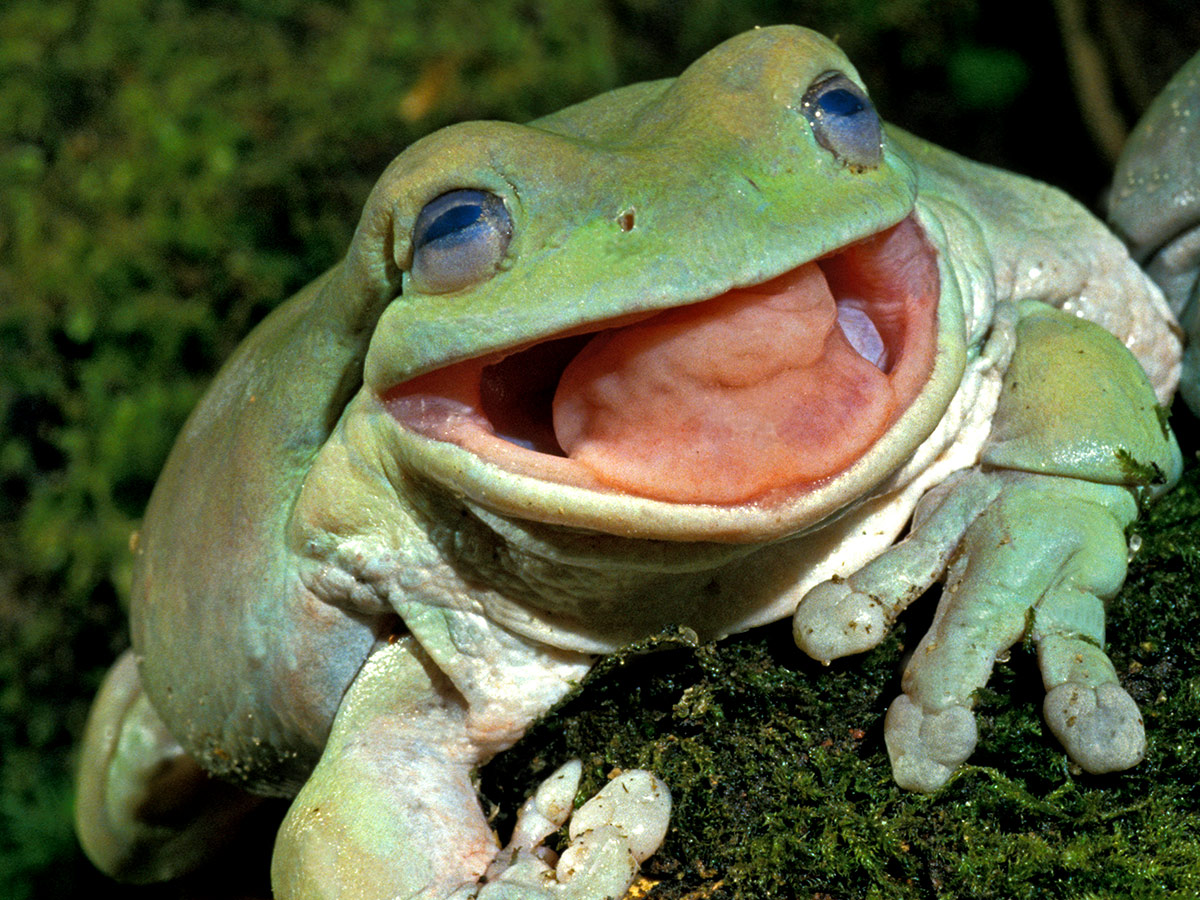
\includegraphics[width=.8\linewidth]{frog}
    \caption{Placeholder image of a frog with a long example caption to show justification setting.}
    \label{fig:frog}
\end{figure}


\begin{SCfigure*}[\sidecaptionrelwidth][t]
    \centering
    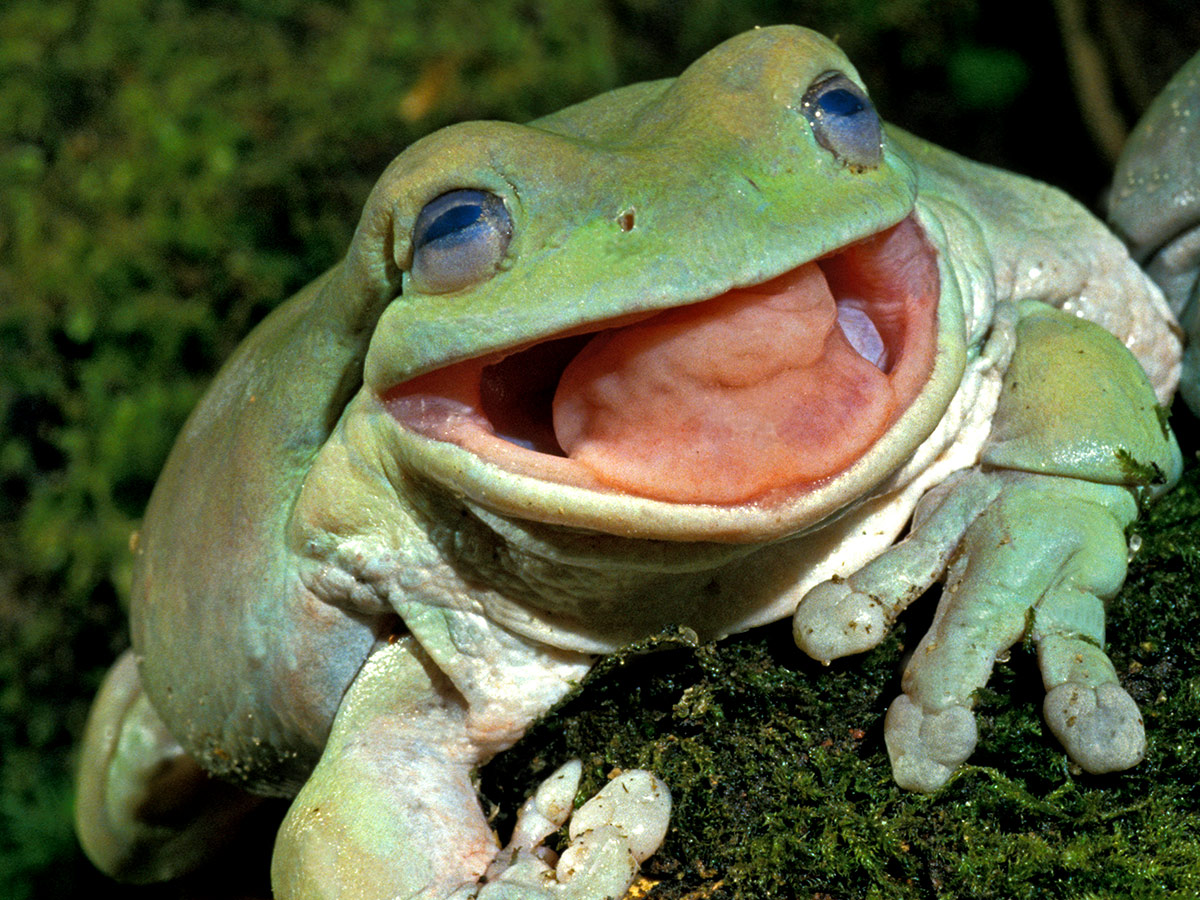
\includegraphics[width=11.4cm,height=11.4cm]{frog}
    \caption{This caption would be placed at the side of the figure, rather than below it.}\label{fig:side}
\end{SCfigure*}
% 
% \subsection*{Digital Figures}
% 
% Only TIFF, EPS, and high-resolution PDF for Mac or PC are allowed for figures that will appear in the main text, and images must be final size. Authors may submit U3D or PRC files for 3D images; these must be accompanied by 2D representations in TIFF, EPS, or high-resolution PDF format.  Color images must be in RGB (red, green, blue) mode. Include the font files for any text. 
% 
% Figures and Tables should be labelled and referenced in the standard way using the \verb|\label{}| and \verb|\ref{}| commands.
% 
% Figure \ref{fig:frog} shows an example of how to insert a column-wide figure. To insert a figure wider than one column, please use the \verb|\begin{figure*}...\end{figure*}| environment. Figures wider than one column should be sized to 11.4 cm or 17.8 cm wide. Use \verb|\begin{SCfigure*}...\end{SCfigure*}| for a wide figure with side captions.
% 
% \subsection*{Tables}
% In addition to including your tables within this manuscript file, PNAS requires that each table be uploaded to the submission separately as a “Table” file.  Please ensure that each table .tex file contains a preamble, the \verb|\begin{document}| command, and the \verb|\end{document}| command. This is necessary so that the submission system can convert each file to PDF.
% 
% \subsection*{Single column equations}
% 
% Authors may use 1- or 2-column equations in their article, according to their preference.
% 
% To allow an equation to span both columns, use the \verb|\begin{figure*}...\end{figure*}| environment mentioned above for figures.
% 
% Note that the use of the \verb|widetext| environment for equations is not recommended, and should not be used. 
% 
% \begin{figure*}[bt!]
%     \begin{align*}
%         (x+y)^3&=(x+y)(x+y)^2\\
%             &=(x+y)(x^2+2xy+y^2) \numberthis \label{eqn:example} \\
%             &=x^3+3x^2y+3xy^3+x^3. 
%     \end{align*}
% \end{figure*}
% 
% 
% \begin{table}%[tbhp]
%     \centering
%     \caption{Comparison of the fitted potential energy surfaces and ab initio benchmark electronic energy calculations}
%     \begin{tabular}{lrrr}
%         Species & CBS & CV & G3 \\
%         \midrule
%         1. Acetaldehyde & 0.0 & 0.0 & 0.0 \\
%         2. Vinyl alcohol & 9.1 & 9.6 & 13.5 \\
%         3. Hydroxyethylidene & 50.8 & 51.2 & 54.0\\
%         \bottomrule
%     \end{tabular}
% 
%     \addtabletext{nomenclature for the TSs refers to the numbered species in the table.}
% \end{table}
% 
% \subsection*{Supporting Information (SI)}
% 
% Authors should submit SI as a single separate PDF file, combining all text, figures, tables, movie legends, and SI references.  PNAS will publish SI uncomposed, as the authors have provided it.  Additional details can be found here: \href{http://www.pnas.org/page/authors/journal-policies}{policy on SI}.  For SI formatting instructions click \href{https://www.pnascentral.org/cgi-bin/main.plex?form_type=display_auth_si_instructions}{here}.  The PNAS Overleaf SI template can be found \href{https://www.overleaf.com/latex/templates/pnas-template-for-supplementary-information/wqfsfqwyjtsd}{here}.  Refer to the SI Appendix in the manuscript at an appropriate point in the text. Number supporting figures and tables starting with S1, S2, etc.
% 
% Authors who place detailed materials and methods in an SI Appendix must provide sufficient detail in the main text methods to enable a reader to follow the logic of the procedures and results and also must reference the SI methods. If a paper is fundamentally a study of a new method or technique, then the methods must be described completely in the main text.
% 
% \subsubsection*{SI Datasets} 
% 
% Supply Excel (.xls), RTF, or PDF files. This file type will be published in raw format and will not be edited or composed.
% 
% 
% \subsubsection*{SI Movies}
% 
% Supply Audio Video Interleave (avi), Quicktime (mov), Windows Media (wmv), animated GIF (gif), or MPEG files and submit a brief legend for each movie in a Word or RTF file. All movies should be submitted at the desired reproduction size and length. Movies should be no more than 10 MB in size.
% 
% 
% \subsubsection*{3D Figures}
% 
% Supply a composable U3D or PRC file so that it may be edited and composed. Authors may submit a PDF file but please note it will be published in raw format and will not be edited or composed.


\matmethods{Please describe your materials and methods here. This can be more than one paragraph, and may contain subsections and equations as required. Authors should include a statement in the methods section describing how readers will be able to access the data in the paper. 

\subsection*{Subsection for Method}
Example text for subsection.
}

\showmatmethods{} % Display the Materials and Methods section

\acknow{Please include your acknowledgments here, set in a single paragraph. Please do not include any acknowledgments in the Supporting Information, or anywhere else in the manuscript.}

\showacknow{} % Display the acknowledgments section

% Bibliography
\bibliography{procedural}

\end{document}
